\documentclass[12pt]{article} 
\usepackage[margin=2cm]{geometry} 
\usepackage{psfrag} 
\usepackage{graphicx} 
\usepackage{epstopdf} 
\usepackage{longtable,booktabs} 
\usepackage{amsmath,amsfonts} 
\usepackage{breqn} 
\usepackage{float,morefloats,caption} 
\begin{document} 
% 24-May-2024 11:52:25, created by McMCDiagnostics.m 
 
\begin{center}
\begin{longtable}{lcc} 
\caption{MCMC Inefficiency factors per block}\\
 \label{Table:MCMC_inefficiency_factors}\\
\toprule 
$Parameter            $	 & 	 $     Block~1$	 & 	 $     Block~2$\\
\midrule \endfirsthead 
\caption{(continued)}\\
 \toprule \\ 
$Parameter            $	 & 	 $     Block~1$	 & 	 $     Block~2$\\
\midrule \endhead 
\midrule \multicolumn{3}{r}{(Continued on next page)} \\ \bottomrule \endfoot 
\bottomrule \endlastfoot 
$ \sigma_{{e_g}}      $	 & 	     555.483	 & 	     559.562 \\ 
$ \sigma_{{e_{ZI}}}   $	 & 	     303.552	 & 	     310.181 \\ 
$ \sigma_{{e_Z}}      $	 & 	     237.682	 & 	     277.491 \\ 
$ \sigma_{{e_N}}      $	 & 	     490.432	 & 	     508.176 \\ 
$ \sigma_{{e_D}}      $	 & 	     330.313	 & 	     347.109 \\ 
$ (\phi)              $	 & 	     743.460	 & 	     745.255 \\ 
$ (\eta)              $	 & 	     745.602	 & 	     743.083 \\ 
$ {\rho_g}            $	 & 	     740.614	 & 	     743.790 \\ 
$ {\rho_Z}            $	 & 	     684.882	 & 	     721.195 \\ 
$ {\rho_{ZI}}         $	 & 	     396.274	 & 	     635.785 \\ 
$ {\rho_N}            $	 & 	     730.380	 & 	     731.053 \\ 
$ {\rho_D}            $	 & 	     739.091	 & 	     742.063 \\ 
\end{longtable}
 \end{center}
% End of TeX file.
 
% 26-Sep-2024 14:04:32, created by stoch_simul.m 
 
\begin{center}
\begin{longtable}{lccccc} 
\caption{MATRIX OF COVARIANCE OF EXOGENOUS SHOCKS}\\
 \label{Table:covar_ex_shocks}\\
\toprule 
$Variables  $	 & 	 $       {e_g}$	 & 	 $       {e_Z}$	 & 	 $    {e_{ZI}}$	 & 	 $       {e_N}$	 & 	 $       {e_D}$\\
\midrule \endfirsthead 
\caption{(continued)}\\
 \toprule \\ 
$Variables  $	 & 	 $       {e_g}$	 & 	 $       {e_Z}$	 & 	 $    {e_{ZI}}$	 & 	 $       {e_N}$	 & 	 $       {e_D}$\\
\midrule \endhead 
\midrule \multicolumn{6}{r}{(Continued on next page)} \\ \bottomrule \endfoot 
\bottomrule \endlastfoot 
${e_g}      $	 & 	    0.000273	 & 	    0.000000	 & 	    0.000000	 & 	    0.000000	 & 	    0.000000 \\ 
${e_Z}      $	 & 	    0.000000	 & 	    0.000001	 & 	    0.000000	 & 	    0.000000	 & 	    0.000000 \\ 
${e_{ZI}}   $	 & 	    0.000000	 & 	    0.000000	 & 	    0.000063	 & 	    0.000000	 & 	    0.000000 \\ 
${e_N}      $	 & 	    0.000000	 & 	    0.000000	 & 	    0.000000	 & 	    0.000189	 & 	    0.000000 \\ 
${e_D}      $	 & 	    0.000000	 & 	    0.000000	 & 	    0.000000	 & 	    0.000000	 & 	    0.000056 \\ 
\end{longtable}
 \end{center}
% End of TeX file.
 
\begin{center}
\begin{longtable}{ccc}
\caption{Endogenous}\\%
\hline%
\multicolumn{1}{c}{\textbf{Variable}} &
\multicolumn{1}{c}{\textbf{\LaTeX}} &
\multicolumn{1}{c}{\textbf{Description}}\\%
\hline\hline%
\endfirsthead
\multicolumn{3}{c}{{\tablename} \thetable{} -- Continued}\\%
\hline%
\multicolumn{1}{c}{\textbf{Variable}} &
\multicolumn{1}{c}{\textbf{\LaTeX}} &
\multicolumn{1}{c}{\textbf{Description}}\\%
\hline\hline%
\endhead
\texttt{Y} & ${Y}$ & output\\
\texttt{C} & ${C}$ & consumption\\
\texttt{I} & ${I}$ & investment\\
\texttt{SR} & ${SR}$ & aggregate share-weighted Solow residual\\
\texttt{K} & ${K}$ & Capital\\
\texttt{K\_C} & ${K_C}$ & Capital:C\\
\texttt{K\_I} & ${K_I}$ & Capital:I\\
\texttt{N} & ${N}$ & Hours\\
\texttt{N\_C} & ${N_C}$ & Hours:C\\
\texttt{N\_I} & ${N_I}$ & Hours:I\\
\texttt{Z\_C} & ${Z_C}$ & Tech:C\\
\texttt{u\_ZI} & $u\_ZI$ & u\_ZI\\
\texttt{Z\_I} & ${Z_I}$ & Tech:I\\
\texttt{theta\_N} & ${\theta_N}$ & Labor disutility\\
\texttt{theta\_D} & ${\theta_D}$ & Shopping disutility\\
\texttt{R\_C} & ${R_C}$ & Capital rental rate:C\\
\texttt{R\_I} & ${R_I}$ & Capital rental rate:I\\
\texttt{W} & ${W}$ & Real wage\\
\texttt{D} & ${D}$ & Shopping effort\\
\texttt{D\_C} & ${D}$ & Shopping effort:C\\
\texttt{D\_I} & ${D}$ & Shopping effort:I\\
\texttt{Gam} & ${\Gamma}$ & Composite utility term\\
\texttt{p\_I} & ${p_I}$ & Relative investment price\\
\texttt{g} & ${g}$ & Output growth rate (labor-augmenting technology)\\
\texttt{util\_C} & $util\_C$ & util\_C\\
\texttt{util\_I} & $util\_I$ & util\_I\\
\texttt{util} & $util$ & util\\
\texttt{log\_Y} & $log\_Y$ & log\_Y\\
\texttt{log\_C} & $log\_C$ & log\_C\\
\texttt{log\_I} & $log\_I$ & log\_I\\
\texttt{log\_N} & $log\_N$ & log\_N\\
\texttt{log\_NC} & $log\_NC$ & log\_NC\\
\texttt{log\_NI} & $log\_NI$ & log\_NI\\
\texttt{log\_Y\_N} & $log\_Y\_N$ & log\_Y\_N\\
\texttt{log\_SR} & $log\_SR$ & log\_SR\\
\texttt{log\_D} & $log\_D$ & log\_D\\
\texttt{log\_p\_I} & $log\_p\_I$ & log\_p\_I\\
\texttt{log\_util} & $log\_util$ & log\_util\\
\texttt{C\_obs} & $C\_obs$ & C\_obs\\
\texttt{I\_obs} & $I\_obs$ & I\_obs\\
\texttt{Y\_obs} & $Y\_obs$ & Y\_obs\\
\texttt{Y\_N\_obs} & $Y\_N\_obs$ & Y\_N\_obs\\
\texttt{SR\_obs} & $SR\_obs$ & SR\_obs\\
\texttt{p\_I\_obs} & $p\_I\_obs$ & p\_I\_obs\\
\texttt{NC\_obs} & $NC\_obs$ & NC\_obs\\
\texttt{NI\_obs} & $NI\_obs$ & NI\_obs\\
\texttt{N\_obs} & $N\_obs$ & N\_obs\\
\texttt{D\_obs} & $D\_obs$ & D\_obs\\
\texttt{util\_obs} & $util\_obs$ & util\_obs\\
\hline%
\end{longtable}
\end{center}
\begin{center}
\begin{longtable}{ccc}
\caption{Exogenous}\\%
\hline%
\multicolumn{1}{c}{\textbf{Variable}} &
\multicolumn{1}{c}{\textbf{\LaTeX}} &
\multicolumn{1}{c}{\textbf{Description}}\\%
\hline\hline%
\endfirsthead
\multicolumn{3}{c}{{\tablename} \thetable{} -- Continued}\\%
\hline%
\multicolumn{1}{c}{\textbf{Variable}} &
\multicolumn{1}{c}{\textbf{\LaTeX}} &
\multicolumn{1}{c}{\textbf{Description}}\\%
\hline\hline%
\endhead
\texttt{e\_g} & ${e_g}$ & TFP shock\\
\texttt{e\_Z} & ${e_Z}$ & TFP shock\\
\texttt{e\_ZI} & ${e_{ZI}}$ & Investment-specific tech shock\\
\texttt{e\_N} & ${e_N}$ & Labor supply shock\\
\texttt{e\_D} & ${e_D}$ & Shopping disutility shock\\
\hline%
\end{longtable}
\end{center}
\begin{center}
\begin{longtable}{ccc}
\caption{Parameters}\\%
\hline%
\multicolumn{1}{c}{\textbf{Variable}} &
\multicolumn{1}{c}{\textbf{\LaTeX}} &
\multicolumn{1}{c}{\textbf{Description}}\\%
\hline\hline%
\endfirsthead
\multicolumn{3}{c}{{\tablename} \thetable{} -- Continued}\\%
\hline%
\multicolumn{1}{c}{\textbf{Variable}} &
\multicolumn{1}{c}{\textbf{\LaTeX}} &
\multicolumn{1}{c}{\textbf{Description}}\\%
\hline\hline%
\endhead
\texttt{sigma} & ${\sigma}$ & Risk aversion\\
\texttt{beta} & ${\beta}$ & Discount factor\\
\texttt{g\_bar} & ${\overline{g}}$ & Quarterly growth rate\\
\texttt{nu} & $(\nu)$ & Frisch elasticity\\
\texttt{I\_Y} & $(I_Y)$ & Investment-output ratio\\
\texttt{K\_Y} & $(K_Y)$ & Capital-output ratio (quarterly)\\
\texttt{labor\_share} & $(labor share)$ & Labor share\\
\texttt{phi} & $(\phi)$ & Shopping matching function elasticity\\
\texttt{eta} & $(\eta)$ & Shopping disutility\\
\texttt{Psi} & $(\Psi)$ & Matching utilization\\
\texttt{rho\_g} & ${\rho_g}$ & persistence shock to labor-augmenting technology growth rate\\
\texttt{rho\_Z} & ${\rho_Z}$ & persistence TFP shock\\
\texttt{rho\_ZI} & ${\rho_{ZI}}$ & persistence I-specific shock\\
\texttt{rho\_N} & ${\rho_N}$ & persistence labor supply shock\\
\texttt{rho\_D} & ${\rho_D}$ & persistence shopping effort shock\\
\texttt{p\_I\_ss} & $p\_I\_ss$ & p\_I\_ss\\
\texttt{N\_ss} & $N\_ss$ & N\_ss\\
\hline%
\end{longtable}
\end{center}
 
\include{BRS_util/latex/BRS_util_latex_parameters} 
\include{BRS_util/latex/BRS_util_priors_table} 
% 30-Sep-2024 16:42:23, created by disp_th_moments.m 
 
\begin{center}
\begin{longtable}{lccccc} 
\caption{COEFFICIENTS OF AUTOCORRELATION}\\
 \label{Table:th_autocorr_matrix}\\
\toprule 
$Order         $	 & 	 $         1$	 & 	 $         2$	 & 	 $         3$	 & 	 $         4$	 & 	 $         5$\\
\midrule \endfirsthead 
\caption{(continued)}\\
 \toprule \\ 
$Order         $	 & 	 $         1$	 & 	 $         2$	 & 	 $         3$	 & 	 $         4$	 & 	 $         5$\\
\midrule \endhead 
\midrule \multicolumn{6}{r}{(Continued on next page)} \\ \bottomrule \endfoot 
\bottomrule \endlastfoot 
$Y\_obs        $	 & 	    0.2383	 & 	    0.2915	 & 	    0.2923	 & 	    0.2932	 & 	    0.2941 \\ 
$Y\_N\_obs     $	 & 	    0.2077	 & 	    0.1497	 & 	    0.1344	 & 	    0.1312	 & 	    0.1308 \\ 
$SR\_obs       $	 & 	    0.0832	 & 	    0.0690	 & 	    0.0595	 & 	    0.0581	 & 	    0.0585 \\ 
$I\_obs        $	 & 	    0.1997	 & 	    0.1229	 & 	    0.1237	 & 	    0.1246	 & 	    0.1254 \\ 
$p\_I\_obs     $	 & 	    0.1108	 & 	    0.1370	 & 	    0.1331	 & 	    0.1292	 & 	    0.1255 \\ 
$C\_obs        $	 & 	    0.2755	 & 	    0.3294	 & 	    0.3300	 & 	    0.3308	 & 	    0.3315 \\ 
$NC\_obs       $	 & 	    0.1805	 & 	    0.1078	 & 	    0.0910	 & 	    0.0874	 & 	    0.0868 \\ 
$NI\_obs       $	 & 	   -0.0137	 & 	    0.0234	 & 	    0.0199	 & 	    0.0198	 & 	    0.0204 \\ 
${\theta_D}    $	 & 	    0.9281	 & 	    0.8614	 & 	    0.7994	 & 	    0.7419	 & 	    0.6886 \\ 
$D\_obs        $	 & 	    0.1067	 & 	    0.0920	 & 	    0.0781	 & 	    0.0756	 & 	    0.0756 \\ 
$util\_obs     $	 & 	    0.1067	 & 	    0.0920	 & 	    0.0781	 & 	    0.0756	 & 	    0.0756 \\ 
$util\_C\_obs  $	 & 	    0.1504	 & 	    0.1092	 & 	    0.0923	 & 	    0.0891	 & 	    0.0889 \\ 
$util\_I\_obs  $	 & 	   -0.0026	 & 	    0.0316	 & 	    0.0267	 & 	    0.0265	 & 	    0.0273 \\ 
\end{longtable}
 \end{center}
% End of TeX file.
 
% 24-May-2024 11:53:17, created by disp_th_moments.m 
 
\begin{center}
\begin{longtable}{lccccccccccc} 
\caption{MATRIX OF CORRELATIONS}\\
 \label{Table:th_corr_matrix}\\
\toprule 
$Variables   $	 & 	 $       Y\_obs$	 & 	 $   Y\_N\_obs$	 & 	 $      SR\_obs$	 & 	 $       I\_obs$	 & 	 $   p\_I\_obs$	 & 	 $       C\_obs$	 & 	 $      NC\_obs$	 & 	 $      NI\_obs$	 & 	 $   {\theta_D}$	 & 	 $       D\_obs$	 & 	 $    util\_obs$\\
\midrule \endfirsthead 
\caption{(continued)}\\
 \toprule \\ 
$Variables   $	 & 	 $       Y\_obs$	 & 	 $   Y\_N\_obs$	 & 	 $      SR\_obs$	 & 	 $       I\_obs$	 & 	 $   p\_I\_obs$	 & 	 $       C\_obs$	 & 	 $      NC\_obs$	 & 	 $      NI\_obs$	 & 	 $   {\theta_D}$	 & 	 $       D\_obs$	 & 	 $    util\_obs$\\
\midrule \endhead 
\midrule \multicolumn{12}{r}{(Continued on next page)} \\ \bottomrule \endfoot 
\bottomrule \endlastfoot 
$Y\_obs      $	 & 	        1.0000	 & 	        0.6741	 & 	        0.7987	 & 	        0.8388	 & 	       -0.0371	 & 	        0.9685	 & 	        0.4161	 & 	        0.6108	 & 	       -0.1983	 & 	        0.7121	 & 	        0.7121 \\ 
$Y\_N\_obs   $	 & 	        0.6741	 & 	        1.0000	 & 	        0.9535	 & 	        0.5641	 & 	       -0.0938	 & 	        0.6535	 & 	       -0.3635	 & 	        0.0121	 & 	       -0.1341	 & 	        0.0978	 & 	        0.0978 \\ 
$SR\_obs     $	 & 	        0.7987	 & 	        0.9535	 & 	        1.0000	 & 	        0.6980	 & 	       -0.0748	 & 	        0.7608	 & 	       -0.1757	 & 	        0.2244	 & 	       -0.1581	 & 	        0.3043	 & 	        0.3043 \\ 
$I\_obs      $	 & 	        0.8388	 & 	        0.5641	 & 	        0.6980	 & 	        1.0000	 & 	       -0.3393	 & 	        0.6769	 & 	        0.2399	 & 	        0.7609	 & 	       -0.2034	 & 	        0.6391	 & 	        0.6391 \\ 
$p\_I\_obs   $	 & 	       -0.0371	 & 	       -0.0938	 & 	       -0.0748	 & 	       -0.3393	 & 	        1.0000	 & 	        0.1049	 & 	        0.0502	 & 	        0.0624	 & 	        0.0545	 & 	        0.0734	 & 	        0.0734 \\ 
$C\_obs      $	 & 	        0.9685	 & 	        0.6535	 & 	        0.7608	 & 	        0.6769	 & 	        0.1049	 & 	        1.0000	 & 	        0.4529	 & 	        0.4779	 & 	       -0.1752	 & 	        0.6706	 & 	        0.6706 \\ 
$NC\_obs     $	 & 	        0.4161	 & 	       -0.3635	 & 	       -0.1757	 & 	        0.2399	 & 	        0.0502	 & 	        0.4529	 & 	        1.0000	 & 	        0.5762	 & 	       -0.0698	 & 	        0.7138	 & 	        0.7138 \\ 
$NI\_obs     $	 & 	        0.6108	 & 	        0.0121	 & 	        0.2244	 & 	        0.7609	 & 	        0.0624	 & 	        0.4779	 & 	        0.5762	 & 	        1.0000	 & 	       -0.1480	 & 	        0.7901	 & 	        0.7901 \\ 
${\theta_D}  $	 & 	       -0.1983	 & 	       -0.1341	 & 	       -0.1581	 & 	       -0.2034	 & 	        0.0545	 & 	       -0.1752	 & 	       -0.0698	 & 	       -0.1480	 & 	        1.0000	 & 	       -0.1589	 & 	       -0.1589 \\ 
$D\_obs      $	 & 	        0.7121	 & 	        0.0978	 & 	        0.3043	 & 	        0.6391	 & 	        0.0734	 & 	        0.6706	 & 	        0.7138	 & 	        0.7901	 & 	       -0.1589	 & 	        1.0000	 & 	        1.0000 \\ 
$util\_obs   $	 & 	        0.7121	 & 	        0.0978	 & 	        0.3043	 & 	        0.6391	 & 	        0.0734	 & 	        0.6706	 & 	        0.7138	 & 	        0.7901	 & 	       -0.1589	 & 	        1.0000	 & 	        1.0000 \\ 
\end{longtable}
 \end{center}
% End of TeX file.
 
% 20-Sep-2024 14:06:39, created by disp_th_moments.m 
 
\begin{center}
\begin{longtable}{lccc} 
\caption{THEORETICAL MOMENTS}\\
 \label{Table:th_moments}\\
\toprule 
$VARIABLE      $	 & 	 $         MEAN$	 & 	 $    STD. DEV.$	 & 	 $     VARIANCE$\\
\midrule \endfirsthead 
\caption{(continued)}\\
 \toprule \\ 
$VARIABLE      $	 & 	 $         MEAN$	 & 	 $    STD. DEV.$	 & 	 $     VARIANCE$\\
\midrule \endhead 
\midrule \multicolumn{4}{r}{(Continued on next page)} \\ \bottomrule \endfoot 
\bottomrule \endlastfoot 
$Y\_obs        $	 & 	       0.0000	 & 	       0.0141	 & 	       0.0002 \\ 
$Y\_N\_obs     $	 & 	       0.0000	 & 	       0.0125	 & 	       0.0002 \\ 
$SR\_obs       $	 & 	       0.0000	 & 	       0.0110	 & 	       0.0001 \\ 
$I\_obs        $	 & 	       0.0000	 & 	       0.0238	 & 	       0.0006 \\ 
$p\_I\_obs     $	 & 	       0.0000	 & 	       0.0101	 & 	       0.0001 \\ 
$C\_obs        $	 & 	       0.0000	 & 	       0.0130	 & 	       0.0002 \\ 
$NC\_obs       $	 & 	       0.0000	 & 	       0.0103	 & 	       0.0001 \\ 
$NI\_obs       $	 & 	       0.0000	 & 	       0.0185	 & 	       0.0003 \\ 
${\theta_D}    $	 & 	       0.0000	 & 	       0.0200	 & 	       0.0004 \\ 
$D\_obs        $	 & 	       0.0000	 & 	       0.0169	 & 	       0.0003 \\ 
$util\_obs     $	 & 	       0.0000	 & 	       0.0149	 & 	       0.0002 \\ 
$util\_C\_obs  $	 & 	       0.0000	 & 	       0.0139	 & 	       0.0002 \\ 
$util\_I\_obs  $	 & 	       0.0000	 & 	       0.0221	 & 	       0.0005 \\ 
\end{longtable}
 \end{center}
% End of TeX file.
 
% 30-Sep-2024 16:42:23, created by disp_th_moments.m 
 
\begin{center}
\begin{longtable}{lccccc} 
\caption{VARIANCE DECOMPOSITION (in percent)}\\
 \label{Table:th_var_decomp_uncond}\\
\toprule 
$              $	 & 	 $       {e_g}$	 & 	 $       {e_Z}$	 & 	 $    {e_{ZI}}$	 & 	 $       {e_N}$	 & 	 $       {e_D}$\\
\midrule \endfirsthead 
\caption{(continued)}\\
 \toprule \\ 
$              $	 & 	 $       {e_g}$	 & 	 $       {e_Z}$	 & 	 $    {e_{ZI}}$	 & 	 $       {e_N}$	 & 	 $       {e_D}$\\
\midrule \endhead 
\midrule \multicolumn{6}{r}{(Continued on next page)} \\ \bottomrule \endfoot 
\bottomrule \endlastfoot 
$Y\_obs        $	 & 	        0.95	 & 	       31.76	 & 	        3.02	 & 	        0.68	 & 	       63.59 \\ 
$Y\_N\_obs     $	 & 	       39.77	 & 	       14.00	 & 	        2.37	 & 	       16.89	 & 	       26.97 \\ 
$SR\_obs       $	 & 	       26.70	 & 	        9.14	 & 	        2.45	 & 	        7.66	 & 	       54.05 \\ 
$I\_obs        $	 & 	        0.23	 & 	       21.38	 & 	       11.70	 & 	        0.53	 & 	       66.16 \\ 
$p\_I\_obs     $	 & 	        0.01	 & 	       24.95	 & 	       62.24	 & 	        0.07	 & 	       12.74 \\ 
$C\_obs        $	 & 	        1.24	 & 	       44.83	 & 	        2.09	 & 	        0.62	 & 	       51.22 \\ 
$NC\_obs       $	 & 	       39.53	 & 	       17.93	 & 	        0.58	 & 	       35.14	 & 	        6.82 \\ 
$NI\_obs       $	 & 	       13.97	 & 	       20.33	 & 	        0.18	 & 	       13.81	 & 	       51.70 \\ 
${\theta_D}    $	 & 	        0.00	 & 	        0.00	 & 	        0.00	 & 	        0.00	 & 	      100.00 \\ 
$D\_obs        $	 & 	       36.59	 & 	        9.37	 & 	        0.53	 & 	        0.20	 & 	       53.31 \\ 
$util\_obs     $	 & 	       36.59	 & 	        9.37	 & 	        0.53	 & 	        0.20	 & 	       53.31 \\ 
$util\_C\_obs  $	 & 	       41.83	 & 	       14.95	 & 	        0.61	 & 	        0.16	 & 	       42.46 \\ 
$util\_I\_obs  $	 & 	       17.78	 & 	       12.31	 & 	        0.24	 & 	        0.29	 & 	       69.38 \\ 
\end{longtable}
 \end{center}
% End of TeX file.
 
\begin{dmath*}
r = \left(1+{{r_ann}}\right)^{0.25}-1.0
\end{dmath*}
\begin{dmath*}
I\_K = \frac{{{I_Y}}}{{{K_Y}}}
\end{dmath*}
\begin{dmath*}
delta = 1+\frac{{{I_Y}}}{{{K_Y}}}-\exp\left({{\overline{g}}}\right)
\end{dmath*}
\begin{dmath*}
alpha\_K = {{K_Y}}\, \left(\left(1+{{r_ann}}\right)^{0.25}-1.0+1+\frac{{{I_Y}}}{{{K_Y}}}-\exp\left({{\overline{g}}}\right)\right)
\end{dmath*}
\begin{dmath*}
beta = \exp\left({{\overline{g}}}\right)^{{{\gamma}}}\, \frac{1}{1+\left(1+{{r_ann}}\right)^{0.25}-1.0}
\end{dmath*}
\begin{dmath*}
sigma\_b = \left(1+{{r_ann}}\right)^{0.25}-1.0+1+\frac{{{I_Y}}}{{{K_Y}}}-\exp\left({{\overline{g}}}\right)
\end{dmath*}
\begin{dmath*}
phi = \frac{\left(1+{{\eta}}\right)\, {{m}}}{1+{{\eta}}\, {{m}}}
\end{dmath*}
\begin{dmath*}
alpha\_N = {(labor share)}\, \left(1-\frac{\left(1+{{\eta}}\right)\, {{m}}}{1+{{\eta}}\, {{m}}}\right)
\end{dmath*}
\begin{dmath*}
D\_ss = \left(\frac{\left(1+{{\eta}}\right)\, {{m}}}{1+{{\eta}}\, {{m}}}\right)^{\frac{{{\eta}}}{1+{{\eta}}}}
\end{dmath*}
\begin{dmath*}
D\_C\_ss = \left(1-{{I_Y}}\right)\, \left(\frac{\left(1+{{\eta}}\right)\, {{m}}}{1+{{\eta}}\, {{m}}}\right)^{\frac{{{\eta}}}{1+{{\eta}}}}
\end{dmath*}
\begin{dmath*}
D\_I\_ss = {{I_Y}}\, \left(\frac{\left(1+{{\eta}}\right)\, {{m}}}{1+{{\eta}}\, {{m}}}\right)^{\frac{{{\eta}}}{1+{{\eta}}}}
\end{dmath*}
\begin{dmath*}
A\_C = \frac{{{\Psi}}}{\left(\left(1-{{I_Y}}\right)\, \left(\frac{\left(1+{{\eta}}\right)\, {{m}}}{1+{{\eta}}\, {{m}}}\right)^{\frac{{{\eta}}}{1+{{\eta}}}}\right)^{\frac{\left(1+{{\eta}}\right)\, {{m}}}{1+{{\eta}}\, {{m}}}}}
\end{dmath*}
\begin{dmath*}
A\_I = \frac{{{\Psi}}}{\left({{I_Y}}\, \left(\frac{\left(1+{{\eta}}\right)\, {{m}}}{1+{{\eta}}\, {{m}}}\right)^{\frac{{{\eta}}}{1+{{\eta}}}}\right)^{\frac{\left(1+{{\eta}}\right)\, {{m}}}{1+{{\eta}}\, {{m}}}}}
\end{dmath*}
\begin{dmath*}
I\_ss = {{I_Y}}
\end{dmath*}
\begin{dmath*}
C\_ss = 1-{{I_Y}}
\end{dmath*}
\begin{dmath*}
K\_ss = {{K_Y}}\, \exp\left({{\overline{g}}}\right)
\end{dmath*}
\begin{dmath*}
K\_I\_ss = {{I_Y}}\, {{K_Y}}\, \exp\left({{\overline{g}}}\right)
\end{dmath*}
\begin{dmath*}
K\_C\_ss = \left(1-{{I_Y}}\right)\, {{K_Y}}\, \exp\left({{\overline{g}}}\right)
\end{dmath*}
\begin{dmath*}
N\_I\_ss = {{I_Y}}\, {N\_ss}
\end{dmath*}
\begin{dmath*}
N\_C\_ss = \left(1-{{I_Y}}\right)\, {N\_ss}
\end{dmath*}
\begin{dmath*}
omega = 1-{{I_Y}}
\end{dmath*}
\begin{dmath*}
W\_ss = \frac{{{I_Y}}\, {(labor share)}\, \left(1-\frac{\left(1+{{\eta}}\right)\, {{m}}}{1+{{\eta}}\, {{m}}}\right)\, \frac{{p\_I\_ss}}{1-\frac{\left(1+{{\eta}}\right)\, {{m}}}{1+{{\eta}}\, {{m}}}}}{{{I_Y}}\, {N\_ss}}
\end{dmath*}
\begin{dmath*}
Z\_C\_ss = \frac{1-{{I_Y}}}{{{\Psi}}\, \exp\left({{\overline{g}}}\right)^{\left(-\left({{K_Y}}\, \left(\left(1+{{r_ann}}\right)^{0.25}-1.0+1+\frac{{{I_Y}}}{{{K_Y}}}-\exp\left({{\overline{g}}}\right)\right)\right)\right)}\, \left(\left(1-{{I_Y}}\right)\, {{K_Y}}\, \exp\left({{\overline{g}}}\right)\right)^{{{K_Y}}\, \left(\left(1+{{r_ann}}\right)^{0.25}-1.0+1+\frac{{{I_Y}}}{{{K_Y}}}-\exp\left({{\overline{g}}}\right)\right)}\, \left(\left(1-{{I_Y}}\right)\, {N\_ss}\right)^{{(labor share)}\, \left(1-\frac{\left(1+{{\eta}}\right)\, {{m}}}{1+{{\eta}}\, {{m}}}\right)}}
\end{dmath*}
\begin{dmath*}
Z\_I\_ss = \frac{{{I_Y}}}{{{\Psi}}\, \exp\left({{\overline{g}}}\right)^{\left(-\left({{K_Y}}\, \left(\left(1+{{r_ann}}\right)^{0.25}-1.0+1+\frac{{{I_Y}}}{{{K_Y}}}-\exp\left({{\overline{g}}}\right)\right)\right)\right)}\, \left({{I_Y}}\, {{K_Y}}\, \exp\left({{\overline{g}}}\right)\right)^{{{K_Y}}\, \left(\left(1+{{r_ann}}\right)^{0.25}-1.0+1+\frac{{{I_Y}}}{{{K_Y}}}-\exp\left({{\overline{g}}}\right)\right)}\, \left({{I_Y}}\, {N\_ss}\right)^{{(labor share)}\, \left(1-\frac{\left(1+{{\eta}}\right)\, {{m}}}{1+{{\eta}}\, {{m}}}\right)}}
\end{dmath*}
\begin{dmath*}
theta\_N\_ss = \frac{\left(1-\frac{\left(1+{{\eta}}\right)\, {{m}}}{1+{{\eta}}\, {{m}}}\right)\, \frac{{{I_Y}}\, {(labor share)}\, \left(1-\frac{\left(1+{{\eta}}\right)\, {{m}}}{1+{{\eta}}\, {{m}}}\right)\, \frac{{p\_I\_ss}}{1-\frac{\left(1+{{\eta}}\right)\, {{m}}}{1+{{\eta}}\, {{m}}}}}{{{I_Y}}\, {N\_ss}}}{{{N}}_{t}^{\frac{1}{{\nu}}}}
\end{dmath*}
% Equation 1
\begin{dmath}
{{N}}_{t}=\left({{N_C}}_{t}^{1+{{\theta}}}\, \left(1-{{I_Y}}\right)^{\left(-{{\theta}}\right)}+{{N_I}}_{t}^{1+{{\theta}}}\, \left(1-\left(1-{{I_Y}}\right)\right)^{\left(-{{\theta}}\right)}\right)^{\frac{1}{1+{{\theta}}}}
\end{dmath}
% Equation 2
\begin{dmath}
{{N}}_{t}^{\frac{1}{{\nu}}}\, \exp\left({{\theta_N}}_{t}\right)\, \frac{\left(1-\frac{\left(1+{{\eta}}\right)\, {{m}}}{1+{{\eta}}\, {{m}}}\right)\, \frac{{{I_Y}}\, {(labor share)}\, \left(1-\frac{\left(1+{{\eta}}\right)\, {{m}}}{1+{{\eta}}\, {{m}}}\right)\, \frac{{p\_I\_ss}}{1-\frac{\left(1+{{\eta}}\right)\, {{m}}}{1+{{\eta}}\, {{m}}}}}{{{I_Y}}\, {N\_ss}}}{{{N}}_{t}^{\frac{1}{{\nu}}}}={{W}}_{t}\, \exp\left({{\theta_C}}_{t}\right)\, \left(1-\frac{\left(1+{{\eta}}\right)\, {{m}}}{1+{{\eta}}\, {{m}}}\right)
\end{dmath}
% Equation 3
\begin{dmath}
\exp\left({{\theta_D}}_{t}\right)\, {{D}}_{t}^{\frac{1}{{{\eta}}}}=\frac{{{C}}_{t}\, \frac{\left(1+{{\eta}}\right)\, {{m}}}{1+{{\eta}}\, {{m}}}\, \exp\left({{\theta_C}}_{t}\right)}{{{D}}_{t}}
\end{dmath}
% Equation 4
\begin{dmath}
\exp\left({{\theta_D}}_{t}\right)\, {{D}}_{t}^{\frac{1}{{{\eta}}}}=\frac{{{I}}_{t}\, {{p_I}}_{t}\, \frac{\left(1+{{\eta}}\right)\, {{m}}}{1+{{\eta}}\, {{m}}}\, \exp\left({{\theta_C}}_{t}\right)}{{{D}}_{t}}
\end{dmath}
% Equation 5
\begin{dmath}
{{\Gamma}}_{t}=\exp\left({{\theta_C}}_{t}\right)\, {{C}}_{t}-\frac{\exp\left({{\theta_D}}_{t}\right)\, {{D}}_{t}^{1+\frac{1}{{{\eta}}}}}{1+\frac{1}{{{\eta}}}}-\frac{{{N}}_{t}^{1+\frac{1}{{\nu}}}\, \exp\left({{\theta_N}}_{t}\right)\, \frac{\left(1-\frac{\left(1+{{\eta}}\right)\, {{m}}}{1+{{\eta}}\, {{m}}}\right)\, \frac{{{I_Y}}\, {(labor share)}\, \left(1-\frac{\left(1+{{\eta}}\right)\, {{m}}}{1+{{\eta}}\, {{m}}}\right)\, \frac{{p\_I\_ss}}{1-\frac{\left(1+{{\eta}}\right)\, {{m}}}{1+{{\eta}}\, {{m}}}}}{{{I_Y}}\, {N\_ss}}}{{{N}}_{t}^{\frac{1}{{\nu}}}}}{1+\frac{1}{{\nu}}}-{{\zeta}}\, {{ha}}_{t}
\end{dmath}
% Equation 6
\begin{dmath}
{{ha}}_{t}=\exp\left({{\theta_C}}_{t}\right)\, {{C}}_{t-1}-\frac{\exp\left({{\theta_D}}_{t}\right)\, {{D}}_{t-1}^{1+\frac{1}{{{\eta}}}}}{1+\frac{1}{{{\eta}}}}-\frac{{{N}}_{t-1}^{1+\frac{1}{{\nu}}}\, \exp\left({{\theta_N}}_{t}\right)\, \frac{\left(1-\frac{\left(1+{{\eta}}\right)\, {{m}}}{1+{{\eta}}\, {{m}}}\right)\, \frac{{{I_Y}}\, {(labor share)}\, \left(1-\frac{\left(1+{{\eta}}\right)\, {{m}}}{1+{{\eta}}\, {{m}}}\right)\, \frac{{p\_I\_ss}}{1-\frac{\left(1+{{\eta}}\right)\, {{m}}}{1+{{\eta}}\, {{m}}}}}{{{I_Y}}\, {N\_ss}}}{{{N}}_{t}^{\frac{1}{{\nu}}}}}{1+\frac{1}{{\nu}}}
\end{dmath}
% Equation 7
\begin{dmath}
{{Q}}_{t}=\frac{{{p_I}}_{t}}{1-\frac{\left(1+{{\eta}}\right)\, {{m}}}{1+{{\eta}}\, {{m}}}}\, \left(1-{{\Psi_K}}\, \left({{x}}_{t}-\frac{{{I_Y}}}{{{K_Y}}}\right)\right)^{\left(-1\right)}
\end{dmath}
% Equation 8
\begin{dmath}
{{Q}}_{t}=\left({{R_C}}_{t+1}\, {{h_C}}_{t+1}+{{Q}}_{t+1}\, \left(1-{{\delta_C}}_{t+1}+{{x}}_{t+1}\, {{\Psi_K}}\, \left({{x}}_{t+1}-\frac{{{I_Y}}}{{{K_Y}}}\right)-\frac{{{\Psi_K}}}{2}\, \left({{x}}_{t+1}-\frac{{{I_Y}}}{{{K_Y}}}\right)^{2}\right)\right)\, \exp\left({{g}}_{t+1}\right)^{\left(-{{\gamma}}\right)}\, \left(\frac{{{\Gamma}}_{t+1}}{{{\Gamma}}_{t}}\right)^{\left(-{{\gamma}}\right)}\, \frac{\exp\left({{\theta_C}}_{t+1}\right)\, \exp\left({{\overline{g}}}\right)^{{{\gamma}}}\, \frac{1}{1+\left(1+{{r_ann}}\right)^{0.25}-1.0}}{\exp\left({{\theta_C}}_{t}\right)}
\end{dmath}
% Equation 9
\begin{dmath}
{{Q}}_{t}=\left({{R_I}}_{t+1}\, {{h_I}}_{t+1}+{{Q}}_{t+1}\, \left(1-{{\delta_I}}_{t+1}+{{x}}_{t+1}\, {{\Psi_K}}\, \left({{x}}_{t+1}-\frac{{{I_Y}}}{{{K_Y}}}\right)-\frac{{{\Psi_K}}}{2}\, \left({{x}}_{t+1}-\frac{{{I_Y}}}{{{K_Y}}}\right)^{2}\right)\right)\, \exp\left({{g}}_{t+1}\right)^{\left(-{{\gamma}}\right)}\, \left(\frac{{{\Gamma}}_{t+1}}{{{\Gamma}}_{t}}\right)^{\left(-{{\gamma}}\right)}\, \frac{\exp\left({{\theta_C}}_{t+1}\right)\, \exp\left({{\overline{g}}}\right)^{{{\gamma}}}\, \frac{1}{1+\left(1+{{r_ann}}\right)^{0.25}-1.0}}{\exp\left({{\theta_C}}_{t}\right)}
\end{dmath}
% Equation 10
\begin{dmath}
{{x}}_{t}=\frac{{{I}}_{t}}{{{K}}_{t-1}}\, \exp\left({{g}}_{t}\right)
\end{dmath}
% Equation 11
\begin{dmath}
{{Q}}_{t}\, {{\delta_C}}_{t}={{R_C}}_{t}
\end{dmath}
% Equation 12
\begin{dmath}
{{Q}}_{t}\, {{\delta_I}}_{t}={{R_I}}_{t}
\end{dmath}
% Equation 13
\begin{dmath}
{{\delta_C}}_{t}=1+\frac{{{I_Y}}}{{{K_Y}}}-\exp\left({{\overline{g}}}\right)+\left({{h_C}}_{t}-1\right)\, \left(\left(1+{{r_ann}}\right)^{0.25}-1.0+1+\frac{{{I_Y}}}{{{K_Y}}}-\exp\left({{\overline{g}}}\right)\right)+\left({{h_C}}_{t}-1\right)^{2}\, \frac{{{\sigma_a}}\, \left(\left(1+{{r_ann}}\right)^{0.25}-1.0+1+\frac{{{I_Y}}}{{{K_Y}}}-\exp\left({{\overline{g}}}\right)\right)}{2}
\end{dmath}
% Equation 14
\begin{dmath}
{{\delta_I}}_{t}=1+\frac{{{I_Y}}}{{{K_Y}}}-\exp\left({{\overline{g}}}\right)+\left({{h_I}}_{t}-1\right)\, \left(\left(1+{{r_ann}}\right)^{0.25}-1.0+1+\frac{{{I_Y}}}{{{K_Y}}}-\exp\left({{\overline{g}}}\right)\right)+\left({{h_I}}_{t}-1\right)^{2}\, \frac{{{\sigma_a}}\, \left(\left(1+{{r_ann}}\right)^{0.25}-1.0+1+\frac{{{I_Y}}}{{{K_Y}}}-\exp\left({{\overline{g}}}\right)\right)}{2}
\end{dmath}
% Equation 15
\begin{dmath}
{{\delta_C}}_{t}=\left(1+{{r_ann}}\right)^{0.25}-1.0+1+\frac{{{I_Y}}}{{{K_Y}}}-\exp\left({{\overline{g}}}\right)+\left({{h_C}}_{t}-1\right)\, {{\sigma_a}}\, \left(\left(1+{{r_ann}}\right)^{0.25}-1.0+1+\frac{{{I_Y}}}{{{K_Y}}}-\exp\left({{\overline{g}}}\right)\right)
\end{dmath}
% Equation 16
\begin{dmath}
{{\delta_I}}_{t}=\left(1+{{r_ann}}\right)^{0.25}-1.0+1+\frac{{{I_Y}}}{{{K_Y}}}-\exp\left({{\overline{g}}}\right)+\left({{h_I}}_{t}-1\right)\, {{\sigma_a}}\, \left(\left(1+{{r_ann}}\right)^{0.25}-1.0+1+\frac{{{I_Y}}}{{{K_Y}}}-\exp\left({{\overline{g}}}\right)\right)
\end{dmath}
% Equation 17
\begin{dmath}
{{C}}_{t}=\exp\left({{Z_C}}_{t}\right)\, \frac{1-{{I_Y}}}{{{\Psi}}\, \exp\left({{\overline{g}}}\right)^{\left(-\left({{K_Y}}\, \left(\left(1+{{r_ann}}\right)^{0.25}-1.0+1+\frac{{{I_Y}}}{{{K_Y}}}-\exp\left({{\overline{g}}}\right)\right)\right)\right)}\, \left(\left(1-{{I_Y}}\right)\, {{K_Y}}\, \exp\left({{\overline{g}}}\right)\right)^{{{K_Y}}\, \left(\left(1+{{r_ann}}\right)^{0.25}-1.0+1+\frac{{{I_Y}}}{{{K_Y}}}-\exp\left({{\overline{g}}}\right)\right)}\, \left(\left(1-{{I_Y}}\right)\, {N\_ss}\right)^{{(labor share)}\, \left(1-\frac{\left(1+{{\eta}}\right)\, {{m}}}{1+{{\eta}}\, {{m}}}\right)}}\, {{D}}_{t}^{\frac{\left(1+{{\eta}}\right)\, {{m}}}{1+{{\eta}}\, {{m}}}}\, \frac{{{\Psi}}}{\left(\left(1-{{I_Y}}\right)\, \left(\frac{\left(1+{{\eta}}\right)\, {{m}}}{1+{{\eta}}\, {{m}}}\right)^{\frac{{{\eta}}}{1+{{\eta}}}}\right)^{\frac{\left(1+{{\eta}}\right)\, {{m}}}{1+{{\eta}}\, {{m}}}}}\, \exp\left({{g}}_{t}\right)^{\left(-\left({{K_Y}}\, \left(\left(1+{{r_ann}}\right)^{0.25}-1.0+1+\frac{{{I_Y}}}{{{K_Y}}}-\exp\left({{\overline{g}}}\right)\right)\right)\right)}\, \left({{h_C}}_{t}\, {{K_C}}_{t-1}\right)^{{{K_Y}}\, \left(\left(1+{{r_ann}}\right)^{0.25}-1.0+1+\frac{{{I_Y}}}{{{K_Y}}}-\exp\left({{\overline{g}}}\right)\right)}\, {{N_C}}_{t}^{{(labor share)}\, \left(1-\frac{\left(1+{{\eta}}\right)\, {{m}}}{1+{{\eta}}\, {{m}}}\right)}
\end{dmath}
% Equation 18
\begin{dmath}
{{I}}_{t}=\exp\left({{g}}_{t}\right)^{\left(-\left({{K_Y}}\, \left(\left(1+{{r_ann}}\right)^{0.25}-1.0+1+\frac{{{I_Y}}}{{{K_Y}}}-\exp\left({{\overline{g}}}\right)\right)\right)\right)}\, \exp\left({{Z_I}}_{t}\right)\, \frac{{{I_Y}}}{{{\Psi}}\, \exp\left({{\overline{g}}}\right)^{\left(-\left({{K_Y}}\, \left(\left(1+{{r_ann}}\right)^{0.25}-1.0+1+\frac{{{I_Y}}}{{{K_Y}}}-\exp\left({{\overline{g}}}\right)\right)\right)\right)}\, \left({{I_Y}}\, {{K_Y}}\, \exp\left({{\overline{g}}}\right)\right)^{{{K_Y}}\, \left(\left(1+{{r_ann}}\right)^{0.25}-1.0+1+\frac{{{I_Y}}}{{{K_Y}}}-\exp\left({{\overline{g}}}\right)\right)}\, \left({{I_Y}}\, {N\_ss}\right)^{{(labor share)}\, \left(1-\frac{\left(1+{{\eta}}\right)\, {{m}}}{1+{{\eta}}\, {{m}}}\right)}}\, {{D}}_{t}^{\frac{\left(1+{{\eta}}\right)\, {{m}}}{1+{{\eta}}\, {{m}}}}\, \frac{{{\Psi}}}{\left({{I_Y}}\, \left(\frac{\left(1+{{\eta}}\right)\, {{m}}}{1+{{\eta}}\, {{m}}}\right)^{\frac{{{\eta}}}{1+{{\eta}}}}\right)^{\frac{\left(1+{{\eta}}\right)\, {{m}}}{1+{{\eta}}\, {{m}}}}}\, \left({{h_I}}_{t}\, {{K_I}}_{t-1}\right)^{{{K_Y}}\, \left(\left(1+{{r_ann}}\right)^{0.25}-1.0+1+\frac{{{I_Y}}}{{{K_Y}}}-\exp\left({{\overline{g}}}\right)\right)}\, {{N_I}}_{t}^{{(labor share)}\, \left(1-\frac{\left(1+{{\eta}}\right)\, {{m}}}{1+{{\eta}}\, {{m}}}\right)}
\end{dmath}
% Equation 19
\begin{dmath}
{{I}}_{t}\, \exp\left({{g}}_{t}\right)=\exp\left({{g}}_{t}\right)\, \left({{K_C}}_{t}+{{K_I}}_{t}\right)-{{K_C}}_{t-1}\, \left(1-{{\delta_C}}_{t}\right)-{{K_I}}_{t-1}\, \left(1-{{\delta_I}}_{t}\right)+\frac{{{\Psi_K}}}{2}\, \left({{x}}_{t}-\frac{{{I_Y}}}{{{K_Y}}}\right)^{2}
\end{dmath}
% Equation 20
\begin{dmath}
{{W}}_{t}\, \left(1-\frac{\left(1+{{\eta}}\right)\, {{m}}}{1+{{\eta}}\, {{m}}}\right)=\frac{{{C}}_{t}\, {(labor share)}\, \left(1-\frac{\left(1+{{\eta}}\right)\, {{m}}}{1+{{\eta}}\, {{m}}}\right)}{{{N_C}}_{t}}
\end{dmath}
% Equation 21
\begin{dmath}
\frac{{{W}}_{t}\, \left(1-\frac{\left(1+{{\eta}}\right)\, {{m}}}{1+{{\eta}}\, {{m}}}\right)}{{{p_I}}_{t}}=\frac{{{I}}_{t}\, {(labor share)}\, \left(1-\frac{\left(1+{{\eta}}\right)\, {{m}}}{1+{{\eta}}\, {{m}}}\right)}{{{N_I}}_{t}}
\end{dmath}
% Equation 22
\begin{dmath}
{{R_C}}_{t}\, \left(1-\frac{\left(1+{{\eta}}\right)\, {{m}}}{1+{{\eta}}\, {{m}}}\right)=\exp\left({{g}}_{t}\right)\, \frac{{{C}}_{t}\, {{K_Y}}\, \left(\left(1+{{r_ann}}\right)^{0.25}-1.0+1+\frac{{{I_Y}}}{{{K_Y}}}-\exp\left({{\overline{g}}}\right)\right)}{{{h_C}}_{t}\, {{K_C}}_{t-1}}
\end{dmath}
% Equation 23
\begin{dmath}
\frac{{{R_I}}_{t}\, \left(1-\frac{\left(1+{{\eta}}\right)\, {{m}}}{1+{{\eta}}\, {{m}}}\right)}{{{p_I}}_{t}}=\exp\left({{g}}_{t}\right)\, \frac{{{I}}_{t}\, {{K_Y}}\, \left(\left(1+{{r_ann}}\right)^{0.25}-1.0+1+\frac{{{I_Y}}}{{{K_Y}}}-\exp\left({{\overline{g}}}\right)\right)}{{{h_I}}_{t}\, {{K_I}}_{t-1}}
\end{dmath}
% Equation 24
\begin{dmath}
{{N}}_{t}={{N_C}}_{t}+{{N_I}}_{t}
\end{dmath}
% Equation 25
\begin{dmath}
{{K}}_{t}={{K_C}}_{t}+{{K_I}}_{t}
\end{dmath}
% Equation 26
\begin{dmath}
{{D}}_{t}={{D}}_{t}+{{D}}_{t}
\end{dmath}
% Equation 27
\begin{dmath}
{{Y}}_{t}={{C}}_{t}+{p\_I\_ss}\, {{I}}_{t}
\end{dmath}
% Equation 28
\begin{dmath}
{{util}}_{t}={{D}}_{t}^{\frac{\left(1+{{\eta}}\right)\, {{m}}}{1+{{\eta}}\, {{m}}}}\, \frac{{{C}}_{t}}{{{Y}}_{t}}\, \frac{{{\Psi}}}{\left(\left(1-{{I_Y}}\right)\, \left(\frac{\left(1+{{\eta}}\right)\, {{m}}}{1+{{\eta}}\, {{m}}}\right)^{\frac{{{\eta}}}{1+{{\eta}}}}\right)^{\frac{\left(1+{{\eta}}\right)\, {{m}}}{1+{{\eta}}\, {{m}}}}}\, {{h_C}}_{t}^{{{K_Y}}\, \left(\left(1+{{r_ann}}\right)^{0.25}-1.0+1+\frac{{{I_Y}}}{{{K_Y}}}-\exp\left({{\overline{g}}}\right)\right)}+{{D}}_{t}^{\frac{\left(1+{{\eta}}\right)\, {{m}}}{1+{{\eta}}\, {{m}}}}\, \frac{{{I}}_{t}}{{{Y}}_{t}}\, \frac{{{\Psi}}}{\left({{I_Y}}\, \left(\frac{\left(1+{{\eta}}\right)\, {{m}}}{1+{{\eta}}\, {{m}}}\right)^{\frac{{{\eta}}}{1+{{\eta}}}}\right)^{\frac{\left(1+{{\eta}}\right)\, {{m}}}{1+{{\eta}}\, {{m}}}}}\, {{h_I}}_{t}^{{{K_Y}}\, \left(\left(1+{{r_ann}}\right)^{0.25}-1.0+1+\frac{{{I_Y}}}{{{K_Y}}}-\exp\left({{\overline{g}}}\right)\right)}
\end{dmath}
% Equation 29
\begin{dmath}
{{g}}_{t}={{\overline{g}}}\, \left(1-{{\rho_g}}\right)+{{\rho_g}}\, {{g}}_{t-1}+{{e_g}}_{t}
\end{dmath}
% Equation 30
\begin{dmath}
{{Z_C}}_{t}={{\rho_Z}}\, {{Z_C}}_{t-1}+{{e_Z}}_{t}
\end{dmath}
% Equation 31
\begin{dmath}
{u\_ZI}_{t}={{\rho_{ZI}}}\, {{Z_I}}_{t-1}+{{e_{ZI}}}_{t}
\end{dmath}
% Equation 32
\begin{dmath}
{{Z_I}}_{t}={{Z_C}}_{t}+{u\_ZI}_{t}
\end{dmath}
% Equation 33
\begin{dmath}
{{\theta_N}}_{t}={{\rho_N}}\, {{\theta_N}}_{t-1}-{{e_N}}_{t}
\end{dmath}
% Equation 34
\begin{dmath}
{{\theta_D}}_{t}={{\rho_D}}\, {{\theta_D}}_{t-1}-{{e_D}}_{t}
\end{dmath}
% Equation 35
\begin{dmath}
{{\theta_C}}_{t}={{\rho_C}}\, {{\theta_C}}_{t-1}+{{e_C}}_{t}
\end{dmath}
% Equation 36
\begin{dmath}
{log\_Y}_{t}=\log\left({{Y}}_{t}\right)-(\log\left(\bar{{Y}}\right))
\end{dmath}
% Equation 37
\begin{dmath}
{log\_C}_{t}=\log\left({{C}}_{t}\right)-(\log\left(\bar{{C}}\right))
\end{dmath}
% Equation 38
\begin{dmath}
{log\_I}_{t}=\log\left({{I}}_{t}\right)-(\log\left(\bar{{I}}\right))
\end{dmath}
% Equation 39
\begin{dmath}
{log\_N}_{t}=\log\left({{N}}_{t}\right)-(\log\left(\bar{{N}}\right))
\end{dmath}
% Equation 40
\begin{dmath}
{log\_NC}_{t}=\log\left({{N_C}}_{t}\right)-(\log\left(\bar{{N_C}}\right))
\end{dmath}
% Equation 41
\begin{dmath}
{log\_NI}_{t}=\log\left({{N_I}}_{t}\right)-(\log\left(\bar{{N_I}}\right))
\end{dmath}
% Equation 42
\begin{dmath}
{log\_Y\_N}_{t}={log\_Y}_{t}-{log\_N}_{t}
\end{dmath}
% Equation 43
\begin{dmath}
{log\_D}_{t}=\log\left({{D}}_{t}\right)-(\log\left(\bar{{D}}\right))
\end{dmath}
% Equation 44
\begin{dmath}
{log\_p\_I}_{t}=\log\left({{p_I}}_{t}\right)-(\bar{log\_p\_I})
\end{dmath}
% Equation 45
\begin{dmath}
{log\_util}_{t}=\log\left({{util}}_{t}\right)-(\log\left(\bar{{util}}\right))
\end{dmath}
% Equation 46
\begin{dmath}
{C\_obs}_{t}={{g}}_{t}+{log\_C}_{t}-{log\_C}_{t-1}-{{\overline{g}}}
\end{dmath}
% Equation 47
\begin{dmath}
{I\_obs}_{t}={{g}}_{t}+{log\_I}_{t}-{log\_I}_{t-1}-{{\overline{g}}}
\end{dmath}
% Equation 48
\begin{dmath}
{Y\_obs}_{t}={{g}}_{t}+{log\_Y}_{t}-{log\_Y}_{t-1}-{{\overline{g}}}
\end{dmath}
% Equation 49
\begin{dmath}
{Y\_N\_obs}_{t}={{g}}_{t}+{log\_Y\_N}_{t}-{log\_Y\_N}_{t-1}-{{\overline{g}}}
\end{dmath}
% Equation 50
\begin{dmath}
{p\_I\_obs}_{t}={log\_p\_I}_{t}-{log\_p\_I}_{t-1}
\end{dmath}
% Equation 51
\begin{dmath}
{N\_obs}_{t}={log\_N}_{t}-{log\_N}_{t-1}
\end{dmath}
% Equation 52
\begin{dmath}
{NC\_obs}_{t}={log\_NC}_{t}-{log\_NC}_{t-1}
\end{dmath}
% Equation 53
\begin{dmath}
{NI\_obs}_{t}={log\_NI}_{t}-{log\_NI}_{t-1}
\end{dmath}
% Equation 54
\begin{dmath}
{util\_obs}_{t}={log\_util}_{t}-{log\_util}_{t-1}
\end{dmath}
 
% TeX eps-loader file generated by McmcDiagnostics.m (Dynare).
% 20-Sep-2024 14:06:22
 
\begin{figure}[H]
\centering 
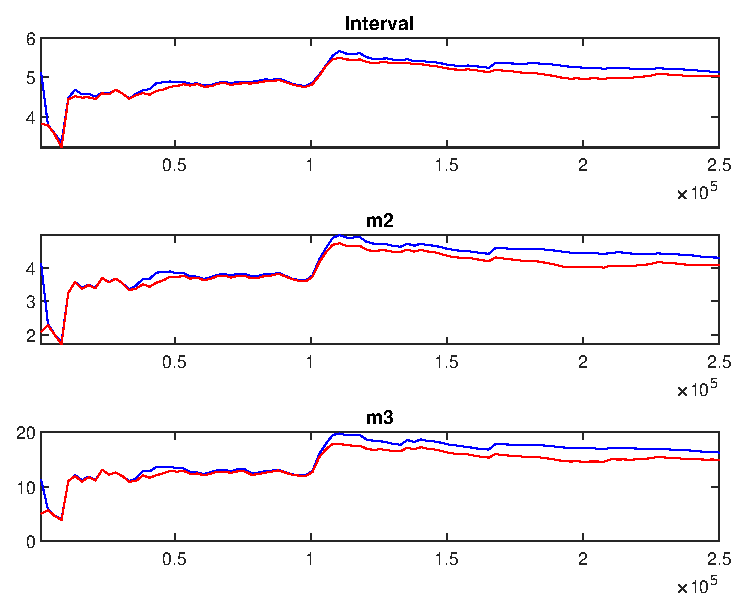
\includegraphics[width=0.8\textwidth]{BRS_util/Output/BRS_util_mdiag}
\caption{Multivariate convergence diagnostics for the Metropolis-Hastings.
The first, second and third rows are respectively the criteria based on
the eighty percent interval, the second and third moments. The different 
parameters are aggregated using the posterior kernel.}\label{Fig:MultivariateDiagnostics}
\end{figure}

% End Of TeX file. 
% TeX-table generated by Dynare.
% RESULTS FROM METROPOLIS HASTINGS (parameters)
% 24-May-2024 11:53:03 
 
\begin{center}
\begin{longtable}{llcccccc} 
\caption{Results from Metropolis-Hastings (parameters)}
 \label{Table:MHPosterior:1}\\
\toprule 
  & \multicolumn{3}{c}{Prior}  &  \multicolumn{4}{c}{Posterior} \\
  \cmidrule(r{.75em}){2-4} \cmidrule(r{.75em}){5-8}
  & Dist. & Mean  & Stdev. & Mean & Stdev. & HPD inf & HPD sup\\
\midrule \endfirsthead 
\caption{(continued)}\\\toprule 
  & \multicolumn{3}{c}{Prior}  &  \multicolumn{4}{c}{Posterior} \\
  \cmidrule(r{.75em}){2-4} \cmidrule(r{.75em}){5-8}
  & Dist. & Mean  & Stdev. & Mean & Stdev. & HPD inf & HPD sup\\
\midrule \endhead 
\bottomrule \multicolumn{8}{r}{(Continued on next page)} \endfoot 
\bottomrule \endlastfoot 
$(\phi)$ & beta &   0.320 & 0.2000 &   0.883& 0.0137 &  0.8628 &  0.9059 \\ 
$(\eta)$ & gamm &   0.200 & 0.1500 &   1.874& 0.0134 &  1.8575 &  1.8985 \\ 
${\rho_g}$ & beta &   0.100 & 0.0500 &   0.228& 0.0067 &  0.2199 &  0.2399 \\ 
${\rho_Z}$ & beta &   0.600 & 0.2000 &   0.972& 0.0039 &  0.9649 &  0.9770 \\ 
${\rho_{ZI}}$ & beta &   0.600 & 0.2000 &   0.999& 0.0011 &  0.9976 &  1.0000 \\ 
${\rho_N}$ & beta &   0.600 & 0.2000 &   0.979& 0.0054 &  0.9708 &  0.9883 \\ 
${\rho_D}$ & beta &   0.600 & 0.2000 &   0.928& 0.0090 &  0.9142 &  0.9408 \\ 
\end{longtable}
 \end{center}
% End of TeX file.
 
% TeX-table generated by Dynare.
% RESULTS FROM METROPOLIS HASTINGS (standard deviation of structural shocks)
% 20-Sep-2024 14:06:32 
 
\begin{center}
\begin{longtable}{llcccccc} 
\caption{Results from Metropolis-Hastings (standard deviation of structural shocks)}
 \label{Table:MHPosterior:2}\\
\toprule 
  & \multicolumn{3}{c}{Prior}  &  \multicolumn{4}{c}{Posterior} \\
  \cmidrule(r{.75em}){2-4} \cmidrule(r{.75em}){5-8}
  & Dist. & Mean  & Stdev. & Mean & Stdev. & HPD inf & HPD sup\\
\midrule \endfirsthead 
\caption{(continued)}\\\toprule 
  & \multicolumn{3}{c}{Prior}  &  \multicolumn{4}{c}{Posterior} \\
  \cmidrule(r{.75em}){2-4} \cmidrule(r{.75em}){5-8}
  & Dist. & Mean  & Stdev. & Mean & Stdev. & HPD inf & HPD sup\\
\midrule \endhead 
\bottomrule \multicolumn{8}{r}{(Continued on next page)} \endfoot 
\bottomrule \endlastfoot 
${e_g}$ & invg &   0.010 & 0.1000 &   0.017& 0.0007 &  0.0153 &  0.0177 \\ 
${e_{ZI}}$ & invg &   0.010 & 0.1000 &   0.008& 0.0004 &  0.0073 &  0.0086 \\ 
${e_Z}$ & invg &   0.010 & 0.1000 &   0.001& 0.0001 &  0.0008 &  0.0010 \\ 
${e_N}$ & invg &   0.010 & 0.1000 &   0.014& 0.0007 &  0.0127 &  0.0148 \\ 
${e_D}$ & invg &   0.010 & 0.1000 &   0.007& 0.0004 &  0.0068 &  0.0081 \\ 
\end{longtable}
 \end{center}
% End of TeX file.
 
% TeX-table generated by dynare_estimation (Dynare).
% RESULTS FROM POSTERIOR MAXIMIZATION (parameters)
% 30-Sep-2024 16:41:25 
 
\begin{center}
\begin{longtable}{llcccc} 
\caption{Results from posterior maximization (parameters)}\\
 \label{Table:Posterior:1}\\
\toprule 
  & \multicolumn{3}{c}{Prior}  &  \multicolumn{2}{c}{Posterior} \\
  \cmidrule(r{.75em}){2-4} \cmidrule(r{.75em}){5-6}
  & Dist. & Mean  & Stdev & Mode & Stdev \\ 
\midrule \endfirsthead 
\caption{(continued)}\\
 \bottomrule 
  & \multicolumn{3}{c}{Prior}  &  \multicolumn{2}{c}{Posterior} \\
  \cmidrule(r{.75em}){2-4} \cmidrule(r{.75em}){5-6}
  & Dist. & Mean  & Stdev & Mode & Stdev \\ 
\midrule \endhead 
\bottomrule \multicolumn{6}{r}{(Continued on next page)}\endfoot 
\bottomrule\endlastfoot 
$(\phi)$ & beta &   0.320 & 0.2000 &   0.8755 &     NaN \\ 
$(\eta)$ & gamm &   0.200 & 0.1500 &   1.8840 &     NaN \\ 
${\rho_g}$ & beta &   0.100 & 0.0500 &   0.2209 &     NaN \\ 
${\rho_Z}$ & beta &   0.600 & 0.2000 &   0.9709 &     NaN \\ 
${\rho_{ZI}}$ & beta &   0.600 & 0.2000 &   0.9994 &     NaN \\ 
${\rho_N}$ & beta &   0.600 & 0.2000 &   0.9816 &     NaN \\ 
${\rho_D}$ & beta &   0.600 & 0.2000 &   0.9275 &     NaN \\ 
\end{longtable}
 \end{center}
% End of TeX file.
 
% TeX-table generated by dynare_estimation (Dynare).
% RESULTS FROM POSTERIOR MAXIMIZATION (standard deviation of structural shocks)
% 20-Sep-2024 14:05:41 
 
\begin{center}
\begin{longtable}{llcccc} 
\caption{Results from posterior maximization (standard deviation of structural shocks)}\\
 \label{Table:Posterior:2}\\
\toprule 
  & \multicolumn{3}{c}{Prior}  &  \multicolumn{2}{c}{Posterior} \\
  \cmidrule(r{.75em}){2-4} \cmidrule(r{.75em}){5-6}
  & Dist. & Mean  & Stdev & Mode & Stdev \\ 
\midrule \endfirsthead 
\caption{(continued)}\\
 \bottomrule 
  & \multicolumn{3}{c}{Prior}  &  \multicolumn{2}{c}{Posterior} \\
  \cmidrule(r{.75em}){2-4} \cmidrule(r{.75em}){5-6}
  & Dist. & Mean  & Stdev & Mode & Stdev \\ 
\midrule \endhead 
\bottomrule \multicolumn{6}{r}{(Continued on next page)}\endfoot 
\bottomrule\endlastfoot 
${e_g}$ & invg &   0.010 & 0.1000 &   0.0165 &     NaN \\ 
${e_{ZI}}$ & invg &   0.010 & 0.1000 &   0.0079 &     NaN \\ 
${e_Z}$ & invg &   0.010 & 0.1000 &   0.0009 &     NaN \\ 
${e_N}$ & invg &   0.010 & 0.1000 &   0.0136 &     NaN \\ 
${e_D}$ & invg &   0.010 & 0.1000 &   0.0074 &     NaN \\ 
\end{longtable}
 \end{center}
% End of TeX file.
 
% TeX eps-loader file generated by PlotPosteriorDistributions.m (Dynare).
% 20-Sep-2024 14:06:35
 
\begin{figure}[H]
\centering
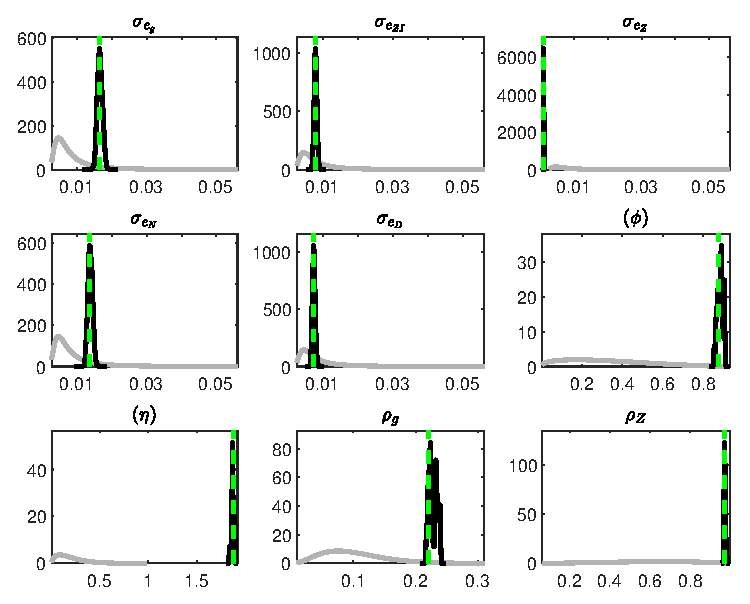
\includegraphics[width=0.80\textwidth]{BRS_util/Output/BRS_util_PriorsAndPosteriors1}
\caption{Priors and posteriors.}\label{Fig:PriorsAndPosteriors:1}
\end{figure}
 
\begin{figure}[H]
\centering
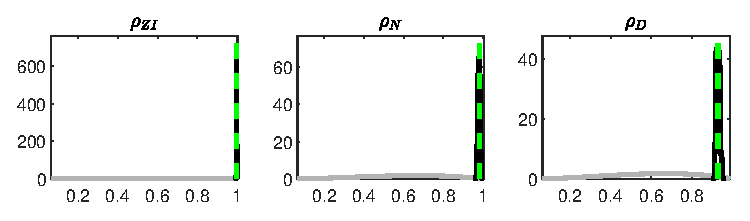
\includegraphics[width=0.80\textwidth]{BRS_util/Output/BRS_util_PriorsAndPosteriors2}
\caption{Priors and posteriors.}\label{Fig:PriorsAndPosteriors:2}
\end{figure}
 
% End of TeX file.
 
\include{BRS_util/Output/BRS_util_UnivariateDiagnostics} 
% TeX eps-loader file generated by mode_check.m (Dynare).
% 26-Sep-2024 14:03:30
 
\begin{figure}[H]
\centering 
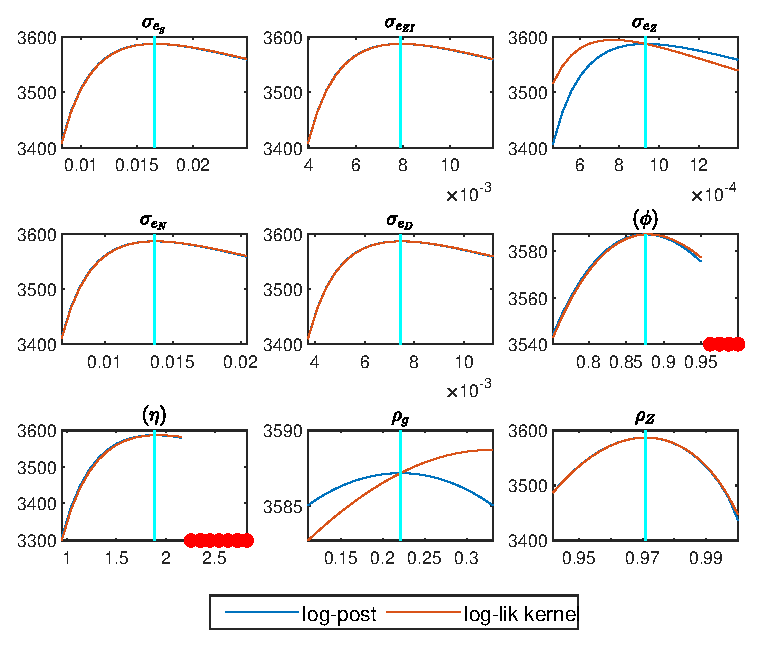
\includegraphics[width=0.80\textwidth]{BRS_util/graphs/BRS_util_CheckPlots1}
\caption{Check plots.}\label{Fig:CheckPlots:1}
\end{figure}
 
\begin{figure}[H]
\centering 
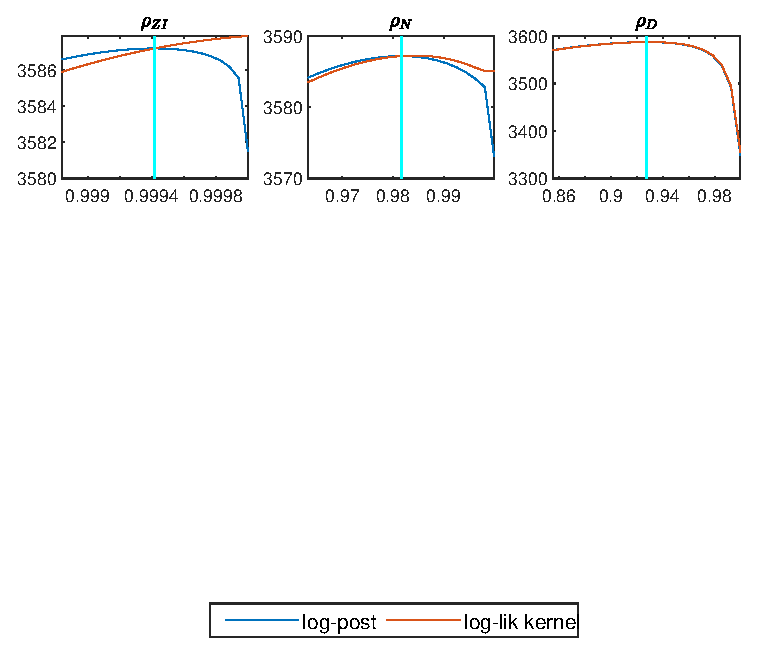
\includegraphics[width=0.80\textwidth]{BRS_util/graphs/BRS_util_CheckPlots2}
\caption{Check plots.}\label{Fig:CheckPlots:2}
\end{figure}
 
 
% TeX eps-loader file generated by dynare_estimation_1.m (Dynare).
% 30-Sep-2024 16:42:22
 
\begin{figure}[H]
\centering 
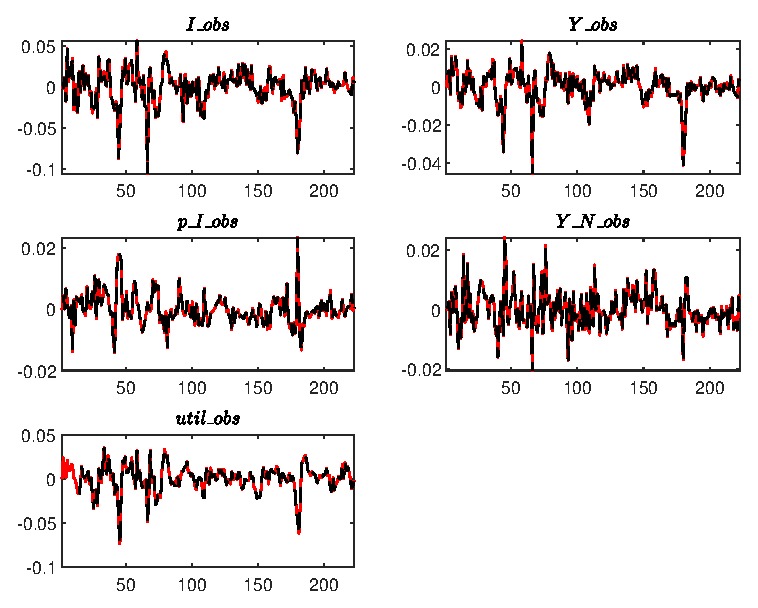
\includegraphics[width=0.80\textwidth]{BRS_util/graphs/BRS_util_HistoricalAndSmoothedVariables1}
\caption{Historical and smoothed variables.}\label{Fig:HistoricalAndSmoothedVariables:1}
\end{figure}


% End of TeX file.
 
% TeX eps-loader file generated by plot_priors.m (Dynare).
% 30-Sep-2024 16:41:17
 
\begin{figure}[H]
\centering
\includegraphics[width=0.80\textwidth]{BRS_util/graphs/BRS_util_Priors1}
\caption{Priors.}\label{Fig:Priors:1}
\end{figure}
\begin{figure}[H]
\centering
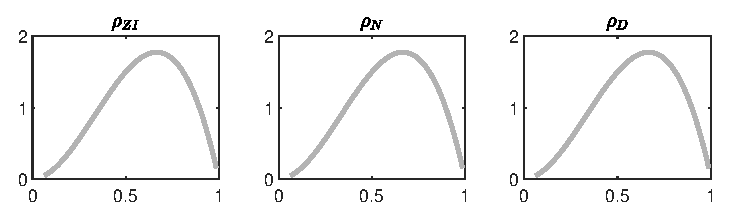
\includegraphics[width=0.80\textwidth]{BRS_util/graphs/BRS_util_Priors2}
\caption{Priors.}\label{Fig:Priors:2}
\end{figure}
 
% End of TeX file.
 
% TeX eps-loader file generated by dynare_estimation_1.m (Dynare).
% 26-Sep-2024 14:04:30
 
\begin{figure}[H]
\centering 
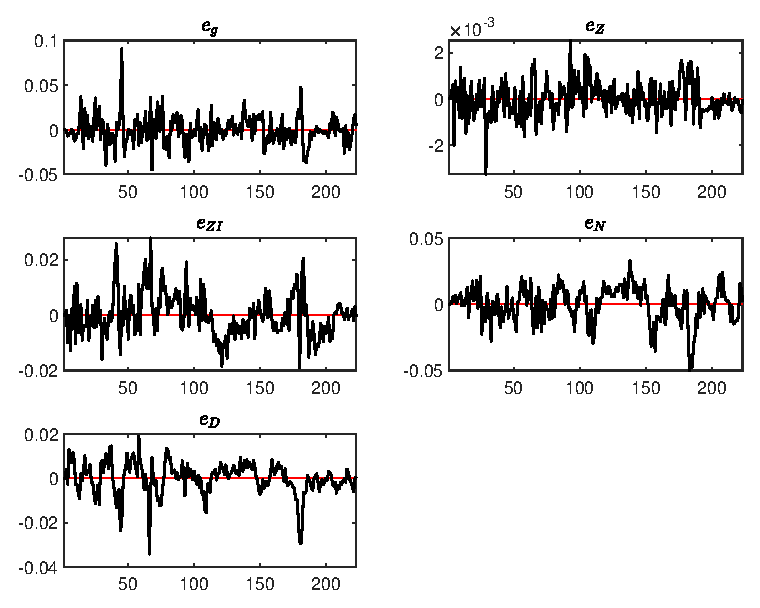
\includegraphics[width=0.80\textwidth]{BRS_util/graphs/BRS_util_SmoothedShocks1}
\caption{Smoothed shocks.}\label{Fig:SmoothedShocks:1}
\end{figure}


% End of TeX file.
 
\end{document} 
